% sage_latex_guidelines.tex V1.20, 14 January 2017

\documentclass[Afour,sagev,times]{sagej}

\usepackage{moreverb,url}

\usepackage[colorlinks,bookmarksopen,bookmarksnumbered,citecolor=red,urlcolor=red]{hyperref}

\newcommand\BibTeX{{\rmfamily B\kern-.05em \textsc{i\kern-.025em b}\kern-.08em
T\kern-.1667em\lower.7ex\hbox{E}\kern-.125emX}}

\def\volumeyear{2016}

%%Vancouver (numbered)
\bibliographystyle{SageV}
\bibliography{paper.bib}

\begin{document}

\runninghead{Charlton and Laudan}

\title{A Web-Based Data Visualization Platform for MATSim}

\author{Billy Charlton\affilnum{1} and Janek Laudan\affilnum{1}}

\affiliation{\affilnum{1}Technische Universit\"at Berlin}

\corrauth{Billy Charlton, Technische Universit\"at Berlin,
Transport Systems Planning and Transport Telematics,
Secretariat SG 12,
Salzufer 17-19, 10587 Berlin, Germany}

\email{charlton@tu-berlin.de}

\begin{abstract}
There are many tools available for analyzing MATSim transport
simulation results, both open-source and commercial. This research
builds a new open-source visualization platform for MATSim outputs that
is entirely web-based. After initial experiments with many different web
technologies, a client/server platform design emerges which leverages
the advanced user interface capabilities of modern browsers on the
front-end, and relies on back-end server processing for more CPU-intensive
tasks. The initial platform is now operational and includes several
aggregate-level visualizations including origin/destination flows,
transit supply, and emissions levels; as well as a fully disaggregate
traffic animation visualization. These visualizations are general
enough to be useful for various projects. Further work is needed
to make them more compelling and the platform more useful for practitioners.
\end{abstract}

\keywords{MATSim, data visualization, agent-based simulation}

\maketitle

\section{Introduction}

MATSim\cite{R1} is an open-source framework for implementing large-scale agent-based transport simulations. MATSim is widely used for transportation research in academic settings, and is gaining momentum as a tool ready for practice in real-world planning contexts.

There are many tools available for analyzing MATSim results, both
open-source and commercial. Typically, analysts can choose either
the free tool OTFVis\cite{R2} or the commercial software
Via \cite{R3}, both of which are desktop software packages requiring installation as well as a fair amount of technical acumen to operate. Alternatives to these tools include the more general-purpose desktop mapping software packages such as QGis and ArcGIS, or statistical software packages, again all of which require installation and expertise to use.

As MATSim moves from the confines of academic research to a more
public-facing role, a notable gap is apparent: there are no web-based interactive tools available for disseminating MATSim data and results. This creates a challenge for using MATSim in public policy settings: the only people who can meaningfully examine and explore results are those who have extensive technical knowledge and access to the specialized software and large datasets involved.

This research explores one way to fill this gap: building an open
web-based data visualization platform which is specifically designed
to complement MATSim.

\section{Motivation}

The rapid advancement of Internet browsing technologies in the last
five years has enabled the web browser to do things much more
"application"-like than ever before: background processing,
three-dimensional rendering using GPU acceleration, offline
support, and more. The combination of these technologies and their
standard implementations on every popular hardware type and operating system now makes the web a very compelling platform.

For MATSim research, the question is: could a web browser really
be useful for exploring and delivering results when the datasets
are so large? Answering this question is the primary motivation for
this research. Essentially, has the web become powerful enough for MATSim?

Currently, analysis of MATSim outputs ends up in research reports, PDFs, video screen-recordings, and presentations. An online dashboard of results which a user could explore and manipulate would not only be more interactive, but might also reveal findings that the original analysts hadn't anticipated.

\section{Requirements}
The research team at Technische Universit\"at Berlin had several
"blank slate" discussions before any code was written: meaning,
if we could start at the very beginning and design something completely web-based and open, what would the bare minimum requirements be for it to be truly useful? The following requirements emerged from those discussions.

\subsection{Requirement 1: Web browser-based}

Given the above-stated motivation and hypothesis that the modern web
platform is ready for large-scale visualization tasks, the most obvious requirement is that the product of this research must work with any modern web browser.

Several specific web technologies developed and made widely available in recent years enable us to perform this research: HTML 5, CSS 3, WebGL, ECMA Script 6, and Web Workers. Briefly, these technologies are:

\begin{enumerate}

\item[(i)] \textbf{HTML 5} improves and standardizes the "document model" of what constitutes a web page and how it is specified.
\item[(i)] \textbf{CSS 3} is a styling language that enables fine-grained layout and styling of individual elements on a page. CSS 3 defines in a consistent, standard way the details of elements including color, size, layout, and animation of page elements.
\item[(ii)] \textbf{WebGL} provides in-browser support for the 3D-accelerated graphics capabilities of modern machines.
\item[(iv)] \textbf{ECMAScript 6} is an updated (2015) version of the venerable Javascript scripting language that has been part of the web platform since the early 1990's. Recent versions of Javascript eliminate the more problematic aspects of the language and make it easier for developers to create bug-free, efficient code.
\item[(v)] \textbf{Web Workers} are a recent (2013) addition to the web platform that allow baiun truly multi-threaded code inside a browser.

\end{enumerate}

A complication in web development is that the major web browser vendors implement these technologies on their own timelines, some much more rapidly than others. Further complicating things is the reality that end users do not always upgrade their browsers frequently (or at all). This creates a landscape where there is a technology adoption curve with a very long "tail". Thus, developers of every web site need to make a conscious decision about where to
draw the line -- choosing necessary technologies for their site to operate correctly, while knowing that some users with older browsers will either have a sub-optimal experience or no access to the site at all.

For this research, we are deliberately exploring the latest \textit{standard} web technologies, with the expectation that access to these technologies will become more and more common in the future. Thus, we are targeting the most recent versions of modern web browsers as of 2019, including Google Chrome, Mozilla Firefox,
and Apple Safari. All three browsers fully support the above-listed technologies, and importantly, all three auto-update automatically, ensuring that most users of those browsers stay current as these technologies evolve.

\subsection{Requirement 2: Open source}

The entire project, including all front-end (browser) and back-end (server) code, must be fully open-source.

No proprietary or closed licensing schemes were considered, primarily because excellent proprietary visualization packages for MATSim already exist. Creating a competing product would be duplicative and unnecessary, and would not further the research goal of determining whether web-based technology is now advanced enough to work with MATSim outputs. The goal of this research is not to replace existing, proprietary solutions, but rather to complement them.

The software developed as part of this research is licensed entirely with the GNU General Public License version 3, commonly known as the \textit{GPL v3}\cite{R4}.

This matches the license of MATSim itself. Several other open-source licenses were considered, including the MIT License and the Apache Public License, but the benefit of sharing a common license with MATSim outweighs any perceived benefits of switching to other open licenses.

\subsection{Requirement 3: Use good defaults, with minimal configuration, and be opinionated}

Since its inception, the web platform has had a relentless focus on simplicity and smooth user onboarding. Users are accustomed to being immediately familiar with a site -- often within seconds of their first interaction. Because of this expectation, it is critical that this research follow current best practices
for user interface (UI) and user experience (UX). Specifically, that means using familiar UI paradigms such as navigation bars and breadcrumbs, separating configuration from usage, limiting settings and options to the bare minimum, and being "opinionated", i.e. encouraging a correct way to accomplish a task.

This approach is dissimilar to some data exploration tools (e.g., QGis and Via) where extreme configurability is emphasized. Rather than providing myriad options for details such as scales and color ramps, our research focuses on choosing good defaults and determining whether that is sufficient for the software to be
useful.

\subsection{Requirement 4: An extensible platform}

Every data visualization use case is different; there is no way to anticipate how the tool will be used. If the platform is too generic, it will be not at all useful. Conversely, if only hard-coded visualizations are created for specific projects, it will be relegated to "demo-ware", meaning it is a successful technology demonstration but not actually useful for real users.

To fulfill this requirement the software platform will need to be extensible: basic capabilities and templates will be provided, but a user with some level of coding skill should be able to create new visualizations that are not anticipated by the researchers.

\section{Initial experiments}

It is no exaggeration to state that the Javascript code library ecosystem is extremely, enormously large. Thousands of libraries and packages are available on a common centralized Javascript repository known as "NPM", and there are often multiple packages that do similar things. As a developer, one must assess and select from these packages or choose to solve a problem by writing code by hand. Of course these libraries are of varying levels of popularity and quality.

Based on the requirements laid out above, some initial experiments were carried out to assess various approaches before committing to a technology stack.

\subsection{Visualizing time-dependent data on a geographic map}

Two popular web-based Javascript libraries were tested for displaying geographic data; Leaflet and Mapbox GL. A simple test case comprised of MATSim simulation outputs was developed, with the goal of displaying aggregated roadway link volumes by time of day.

Leaflet (\url{leafletjs.com}) is very popular and its application programming interface (API) is a bit simpler than that of Mapbox GL. Leaflet uses background map "tiles" at specific zoom levels, and layers data on top of those base maps. With small networks (we tested Cottbus, Germany, a small city of 100,000 inhabitants) Leaflet performed well, but medium-sized and large-sized networks with many elements visible at once suffered from noticeable performance degradation. This was problematic, as this was the simplest use-case envisioned.

Mapbox GL (\url{mapbox.com}) fared much better, apparently better-suited to displaying large datasets with many visible features simultaneously. In addition, Mapbox GL's use of 3D vector graphic mapping instead of preset tiles made for a much more pleasing user experience, with smooth animations between zoom levels and better background processing during page loads. For these reasons, Mapbox GL was chosen as the base map for the remaining geographic visualizations.

\subsection{Visualizing non-geographic data}

There are hundreds of data visualization libraries available for the web which provide ways to produce charts and plots of varying complexity. Our requirement of using open-source code narrows the field considerably.

After experimenting with several packages including D3, Raphael, Morris and others, the package Vega-Lite\cite{R5} exhibited many of the characteristics desired. Notably, Vega-Lite follows a declarative syntax known as the "grammar of graphics", as popularized by Wilkinson\cite{R6}. This grammar allows concise description of the meaningful components of a graphic. An added benefit is that graphs and charts can be downloaded in image format or in Vega source format, which is helpful for other researchers wanting to learn how to use the data format.

\subsection{Dealing with large datasets}

MATSim network files are small enough to fit in RAM, but MATSim plan files and event files can be much larger than RAM, necessitating careful consideration about how to handle them.

Modern browsers allow access via API to a data storage area that is unique per hostname, i.e. http://mysite.com is allowed some storage on the local machine. Initial experiments revealed that each browser vendor implements this storage differently, with very strict limits on the absolute amount storage available, sometimes based on how much free space remains on the user's machine. It became apparent that this local browser-based storage would not be sufficient for MATSim outputs. Running a local file-server process would allow browser access to a specific folder on the machine, which might be nice for advanced analysts but violates the research goal of being fully web-based on the client end. Thus, a client-server paradigm emerges as the only truly viable alternative, and indeed this is how most websites operate today: the browser is the front-end to the heavier processing and storage tasks that happen on someone else's server. Note that "someone else's server" is usually referred to as "the cloud".

\section{Platform architecture}

A client/server architecture was chosen for this research based on the initial experiments described above.

The research team authored back-end server software for file storage, user authentication, and data pre-processing. Due to space considerations, this paper does not delve into the details of those components. Suffice it to mention that the front-end communicates with them to establish what resources a user has access to, and provides an application programming interface, or API, with which to query and fetch available files and resources. The code for those servers is also open source, and may be the subject of future papers.

The front-end architecture has several interacting components, described below.

\subsection{"Vue" Single Page Application}

The primary framework used to build the application is known as "Vue JS" (Vue, available at vuejs.org). Vue is a framework for building interactive user interfaces on the web; essentially it provides the glue between the items a user clicks and the code that runs when they do so. Vue provides many services which allow a web page to behave more like a full-featured application, including state management, routing between different URLs, and componentization of code in a way that encourages code reuse and loose coupling. Vue depends on Javascript, which means it does not work on for users who have disabled scripting in their browser.

Vue is most often used to write so-called "single page applications" which are websites that behave like desktop applications. Most large, popular websites such as Github, Twitter, and Facebook all employ this paradigm, meaning the site handles page transitions and URL's as if they are all in one common namespace, and the user thinks less about visiting URLs and more about navigation through visual components to accomplish tasks. This matches our use case.

Vue components each encapsulate the three elements required for the modern web: HTML layout, Javascript code, and CSS formatting. Components only interact with each other through well-defined pathways of properties and events, which greatly improves debuggability.

\subsection{Build system}

The build system of a modern web application is fairly complex and the Javascript ecosystem changes rapidly. After numerous iterations, the current build system comprises a series of individual tools that all work together to produce the final assets that get sent to a user's browser. Those tools include the Vue command line interface (CLI), the NPM package manager, webpack, babel, and TypeScript.

Notably, the initial codebase was migrated to the Typescript language midway through development, as the benefits of a strongly-typed language were perceived to be worth the development time. TypeScript is a separate language from JavaScript, and enforces type annotations for variables and adds additional features such as enumerations. The TypeScript compiler then converts TypeScript code into ECMAScript 6 JavaScript, which can be run in the browser (as JavaScript is the only scripting language that browsers support).

\subsection{Visualization plug-ins}

One of the main requirements of this research is to produce a system where new visualizations can be produced rapidly and added into the existing framework to generate new capabilities.

The Vue component architecture enables this. To create a new visualization, a developer copies an existing "blank" visualization template and gives it a new name, specifies the file inputs and parameters required, and then uses the above-described libraries to modify the code per their needs.

This currently requires ample coding skill in Javascript; it is not a system that is point-and-click like an online data exploration tool. Experience with other similarly-designed platforms suggests that software-minded analysts or modelers would be able to extend the platform, but typical end users will not.

\section{Results: the current state of the tool}

A working instance of the platform is now online and available at \url{viz.vsp.tu-berlin.de}. Sample datasets are uploaded, and pre-built visualizations are publicly accessible, as a demonstration of the platform's current state. There is also a user login system so that internal researchers can extend and experiment with the system, without exposing data or work-in-progress to the public.

Basic user, project, and file management capabilities are operational. This includes grouping files by model run or by other user-defined tags, as can be seen in Figure~\ref{F1}.

\begin{figure}
\centering
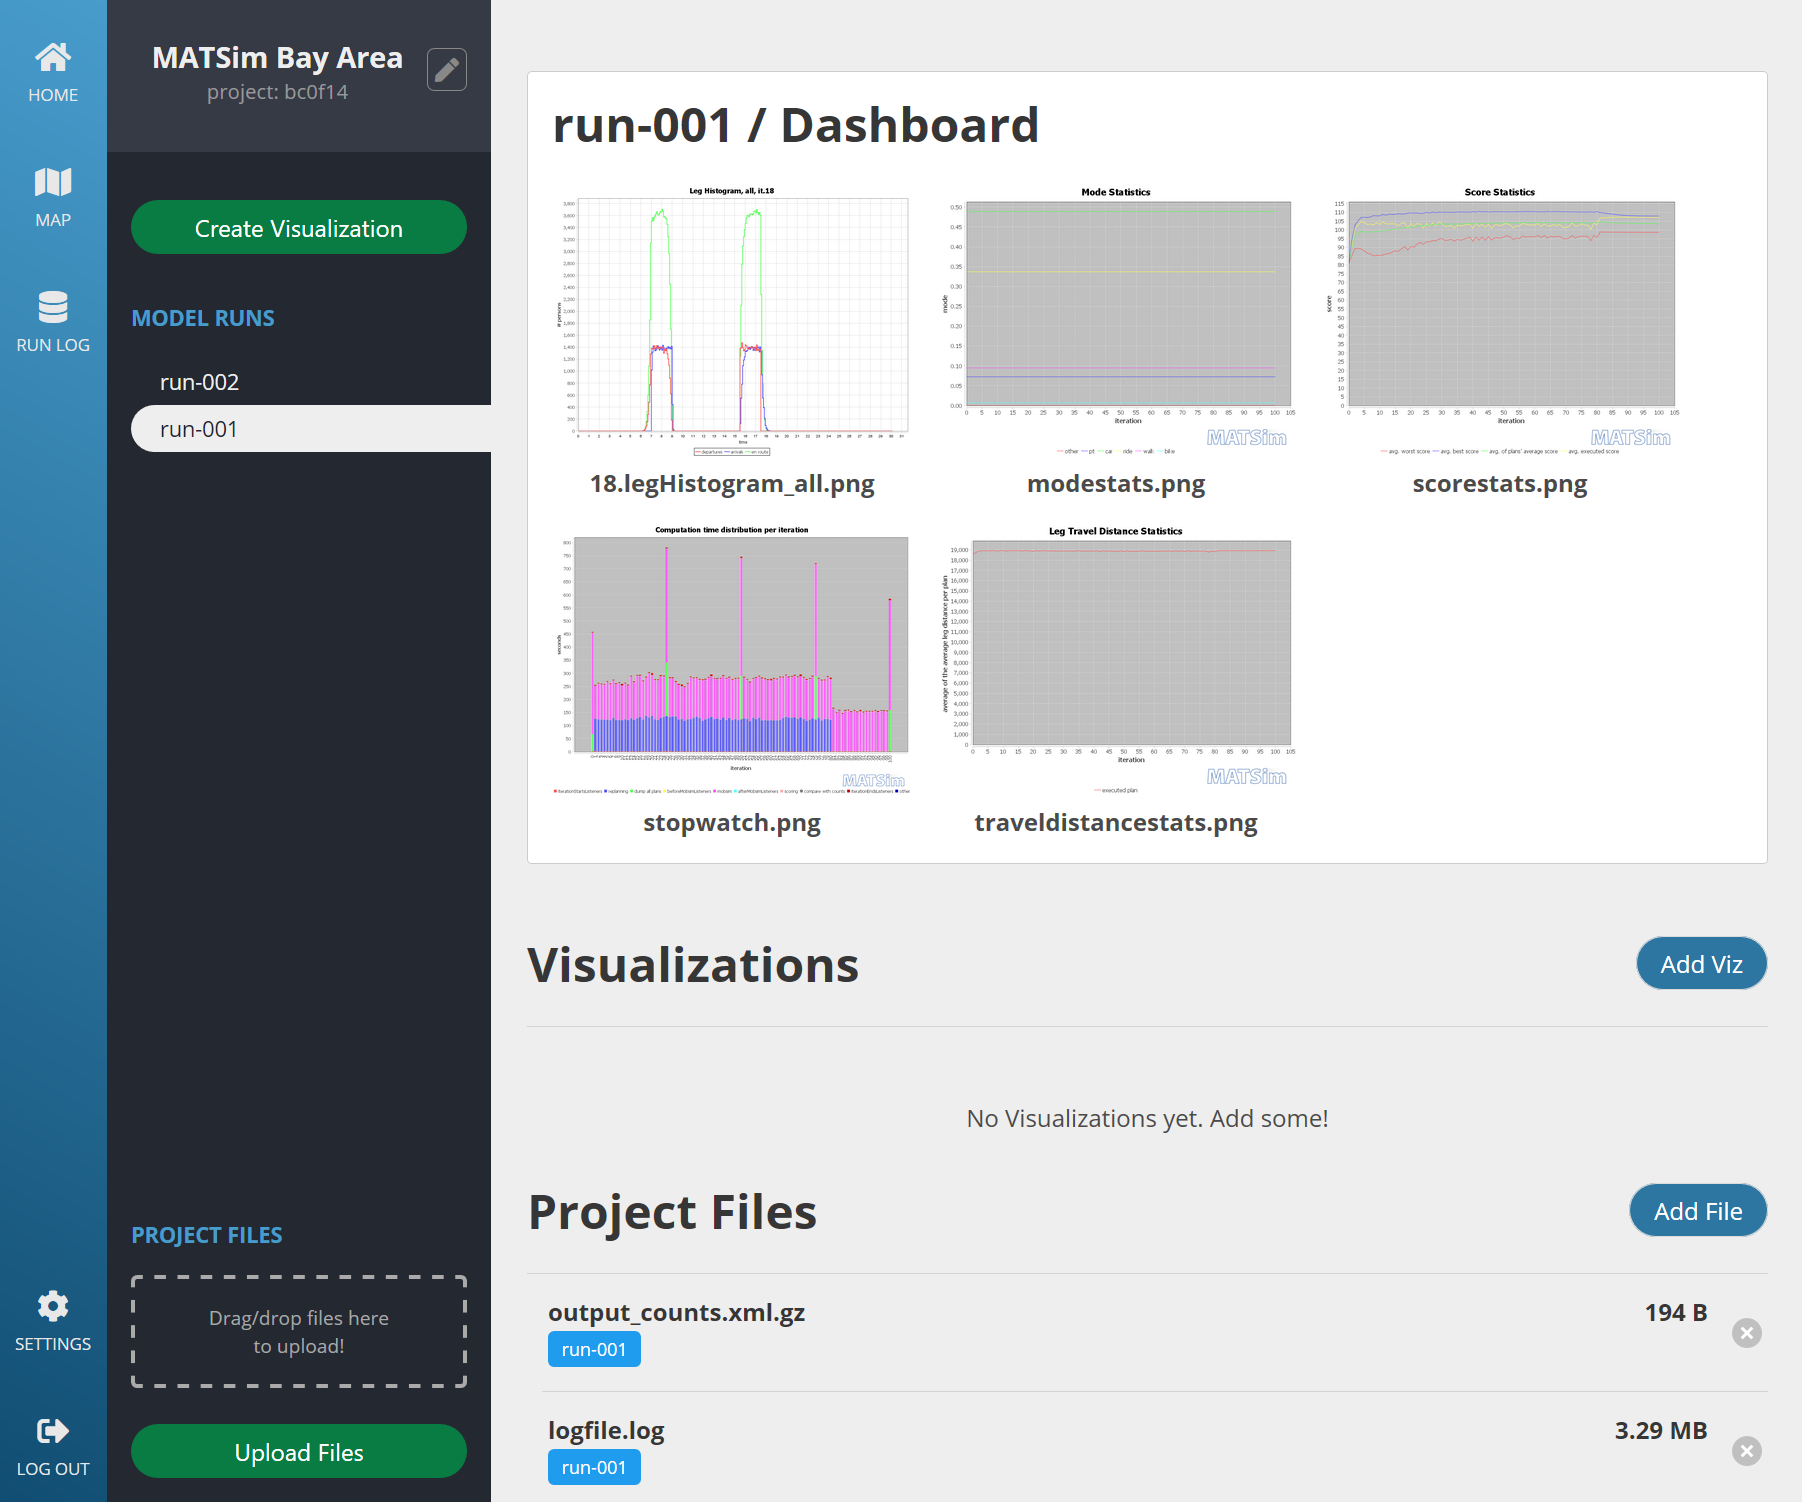
\includegraphics[width=3.25in]{fig-dashboard.png}
\caption{Project dashboard}\label{F1}
\end{figure}

See the following screenshots in Figures~\ref{Fod}-~\ref{Fanim} for examples of the current state of the user interface. Note of course that the tool demos better live than in screenshots, as the whole point of this research is to develop an interactive tool.

Several types of aggregate visualizations are developed:

\begin{enumerate}

\item[(i)] Origin/destination flows between aggregate areas, so called "spider diagrams" (Figure~\ref{Fod})
\item[(i)] Link flows, by time of day and mode (Figure~\ref{Flinkvols})
\item[(iii)] Transit supply explorer, which displays all transit routes and allows the user to see which routes serve specific stops and links. (Figure~\ref{Ftransit})
\item[(iv)] Sankey diagrams, which can be used to depict changes/flows between between scenarios across multiple choices, such as shifts in mode between two scenarios (Figure~\ref{Fsankey})
\item[(v)] Emissions levels on a geographic hexagonal grid basis

\end{enumerate}

\begin{figure}
\centering
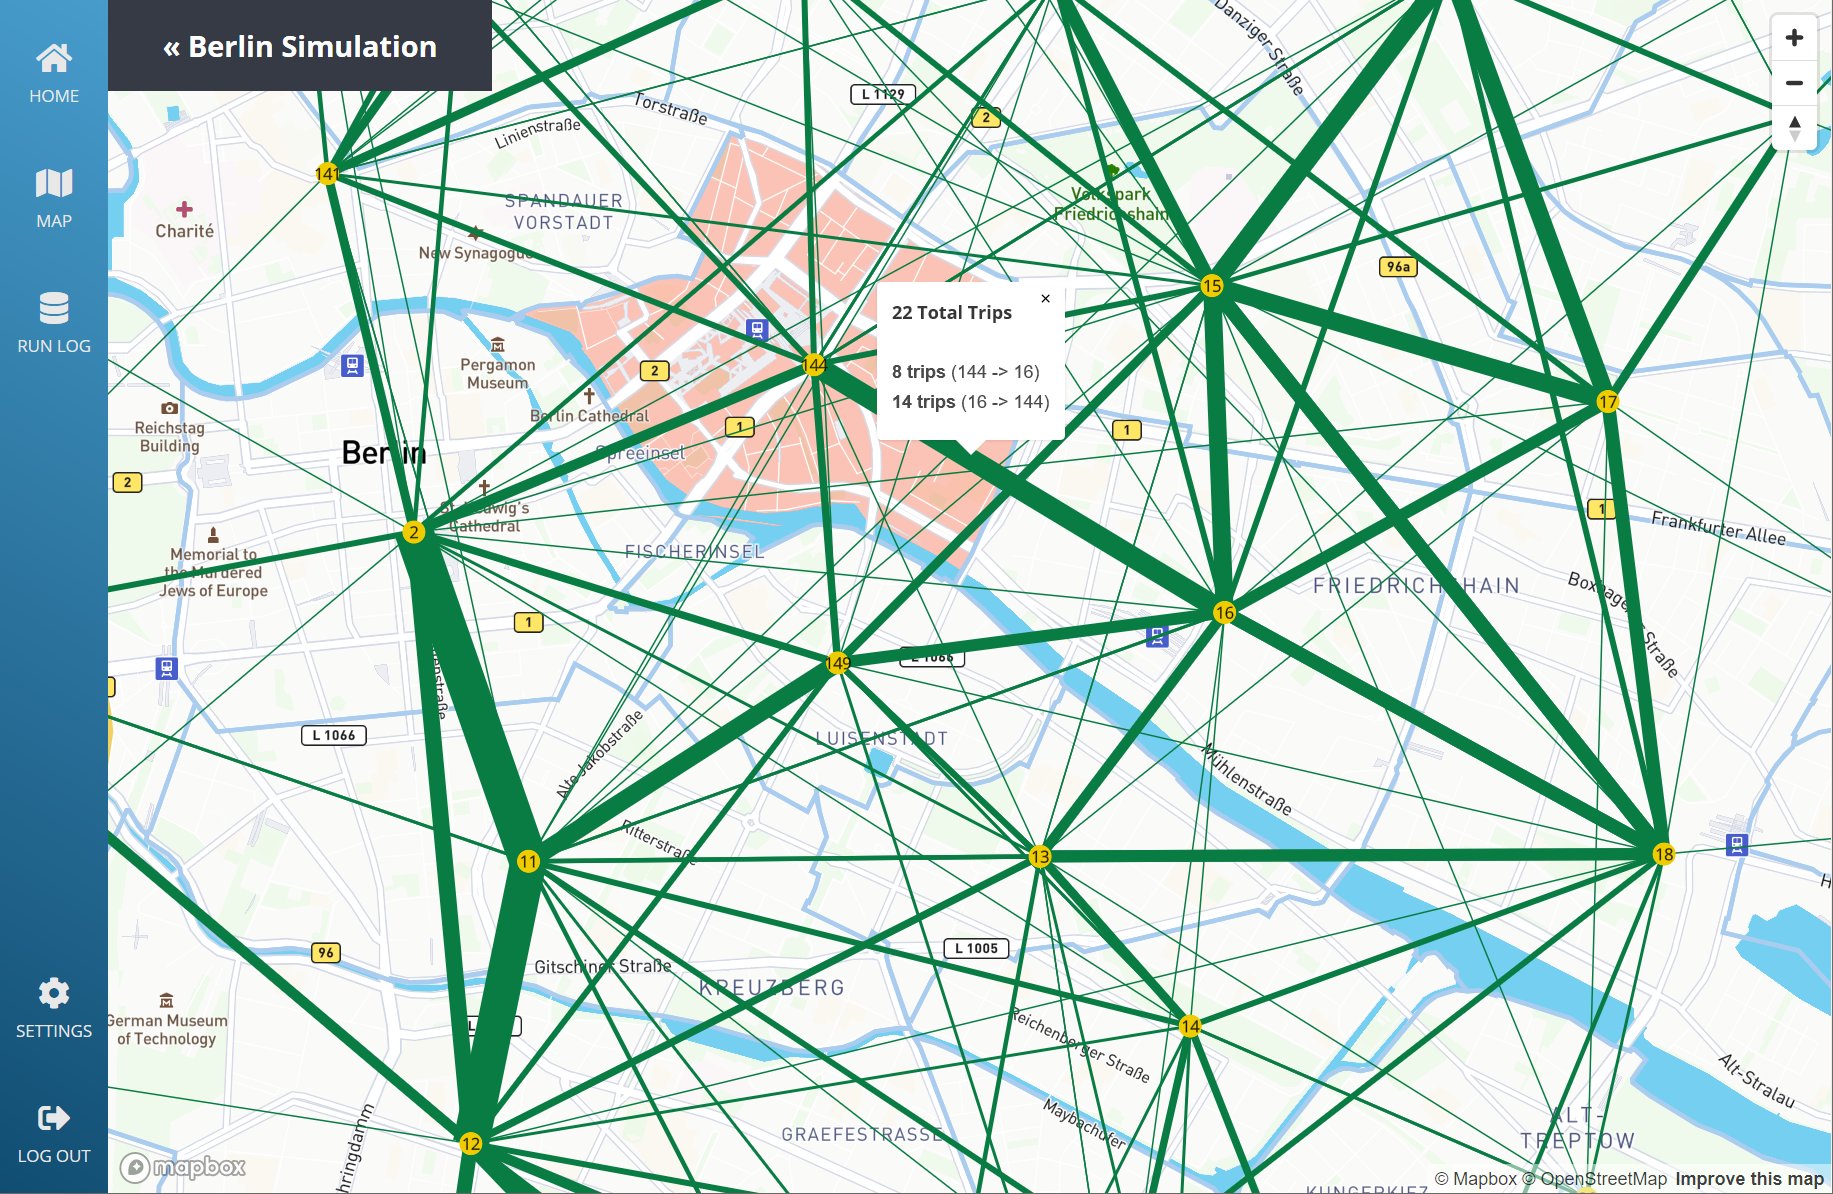
\includegraphics[width=3.25in]{fig-odflow.png}
\caption{Origin/Destination flows}\label{Fod}
\end{figure}

\begin{figure}
\centering
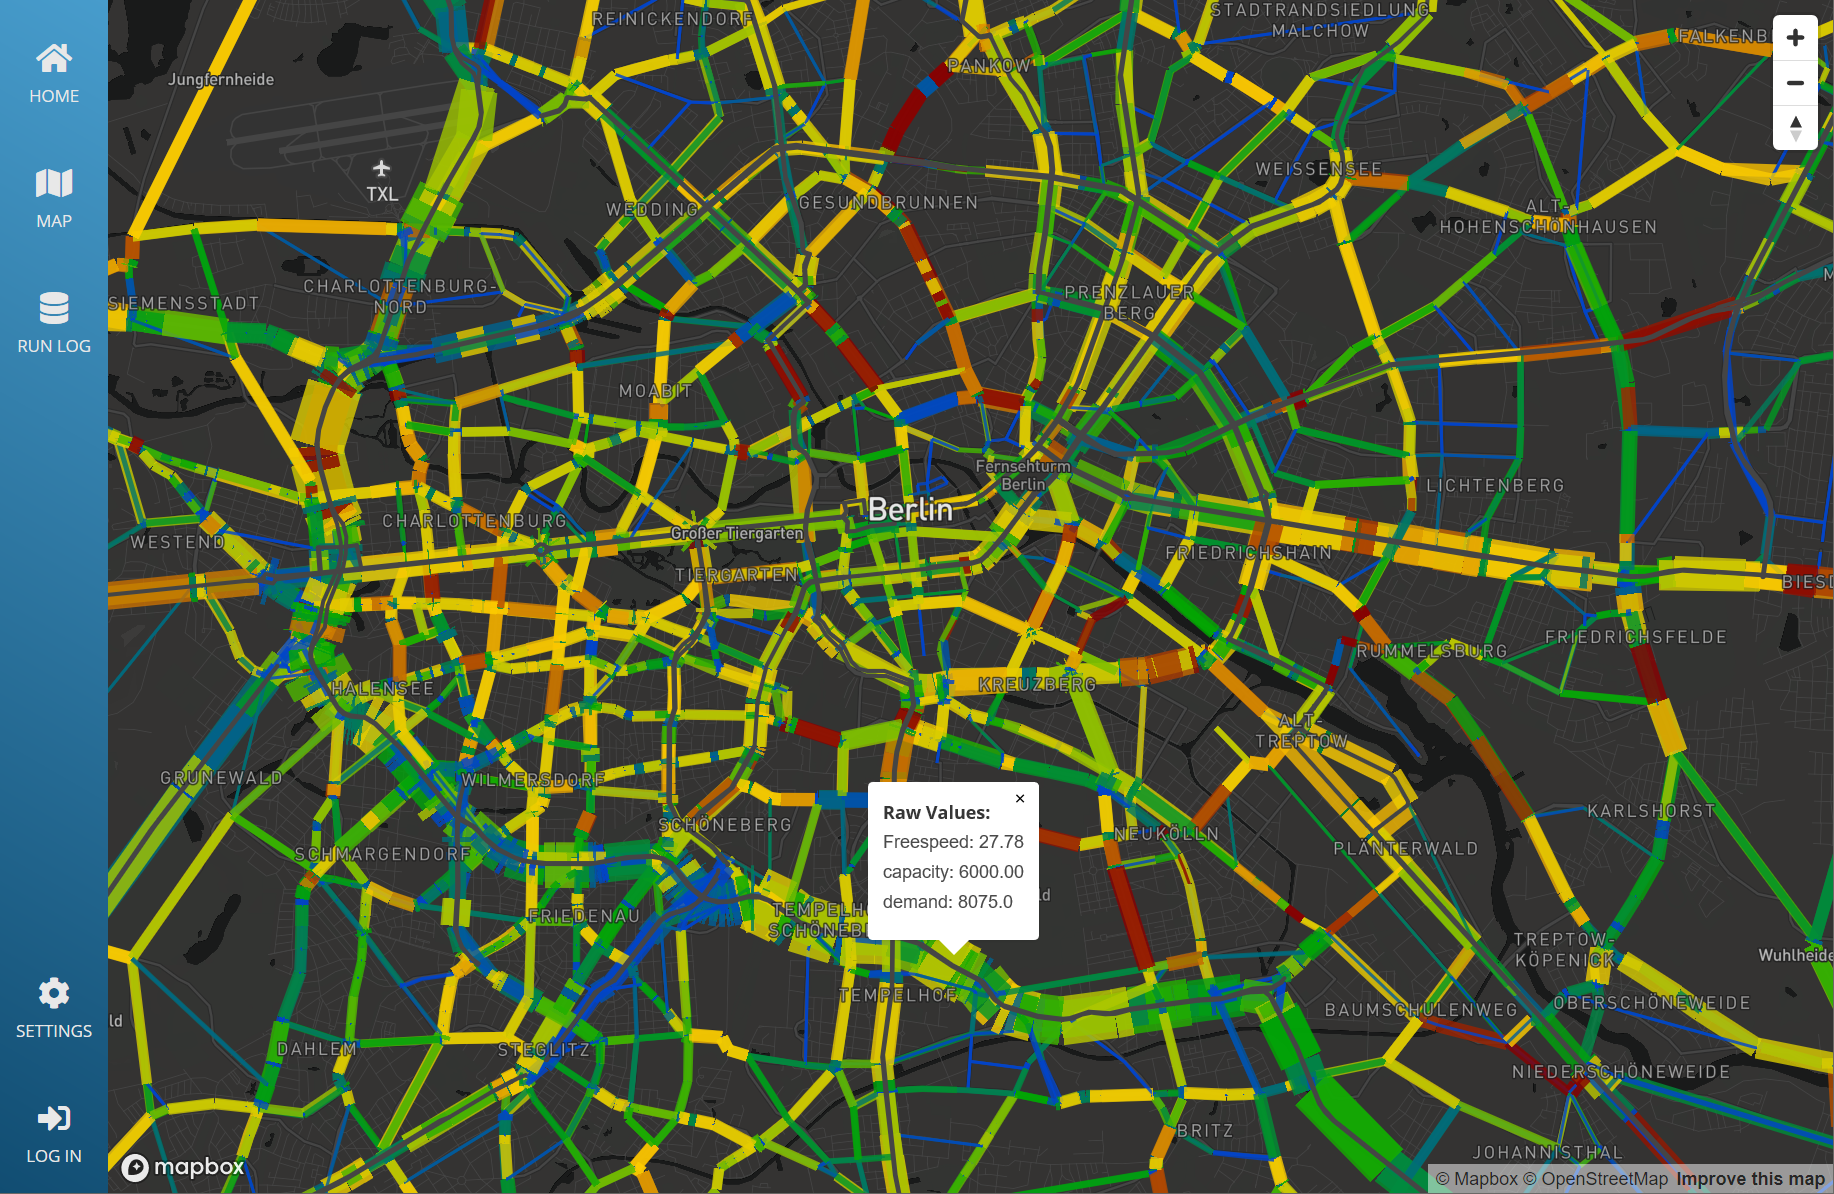
\includegraphics[width=3.25in]{fig-linkvols.png}
\caption{Link volume summary}\label{Flinkvols}
\end{figure}

\begin{figure}
\centering
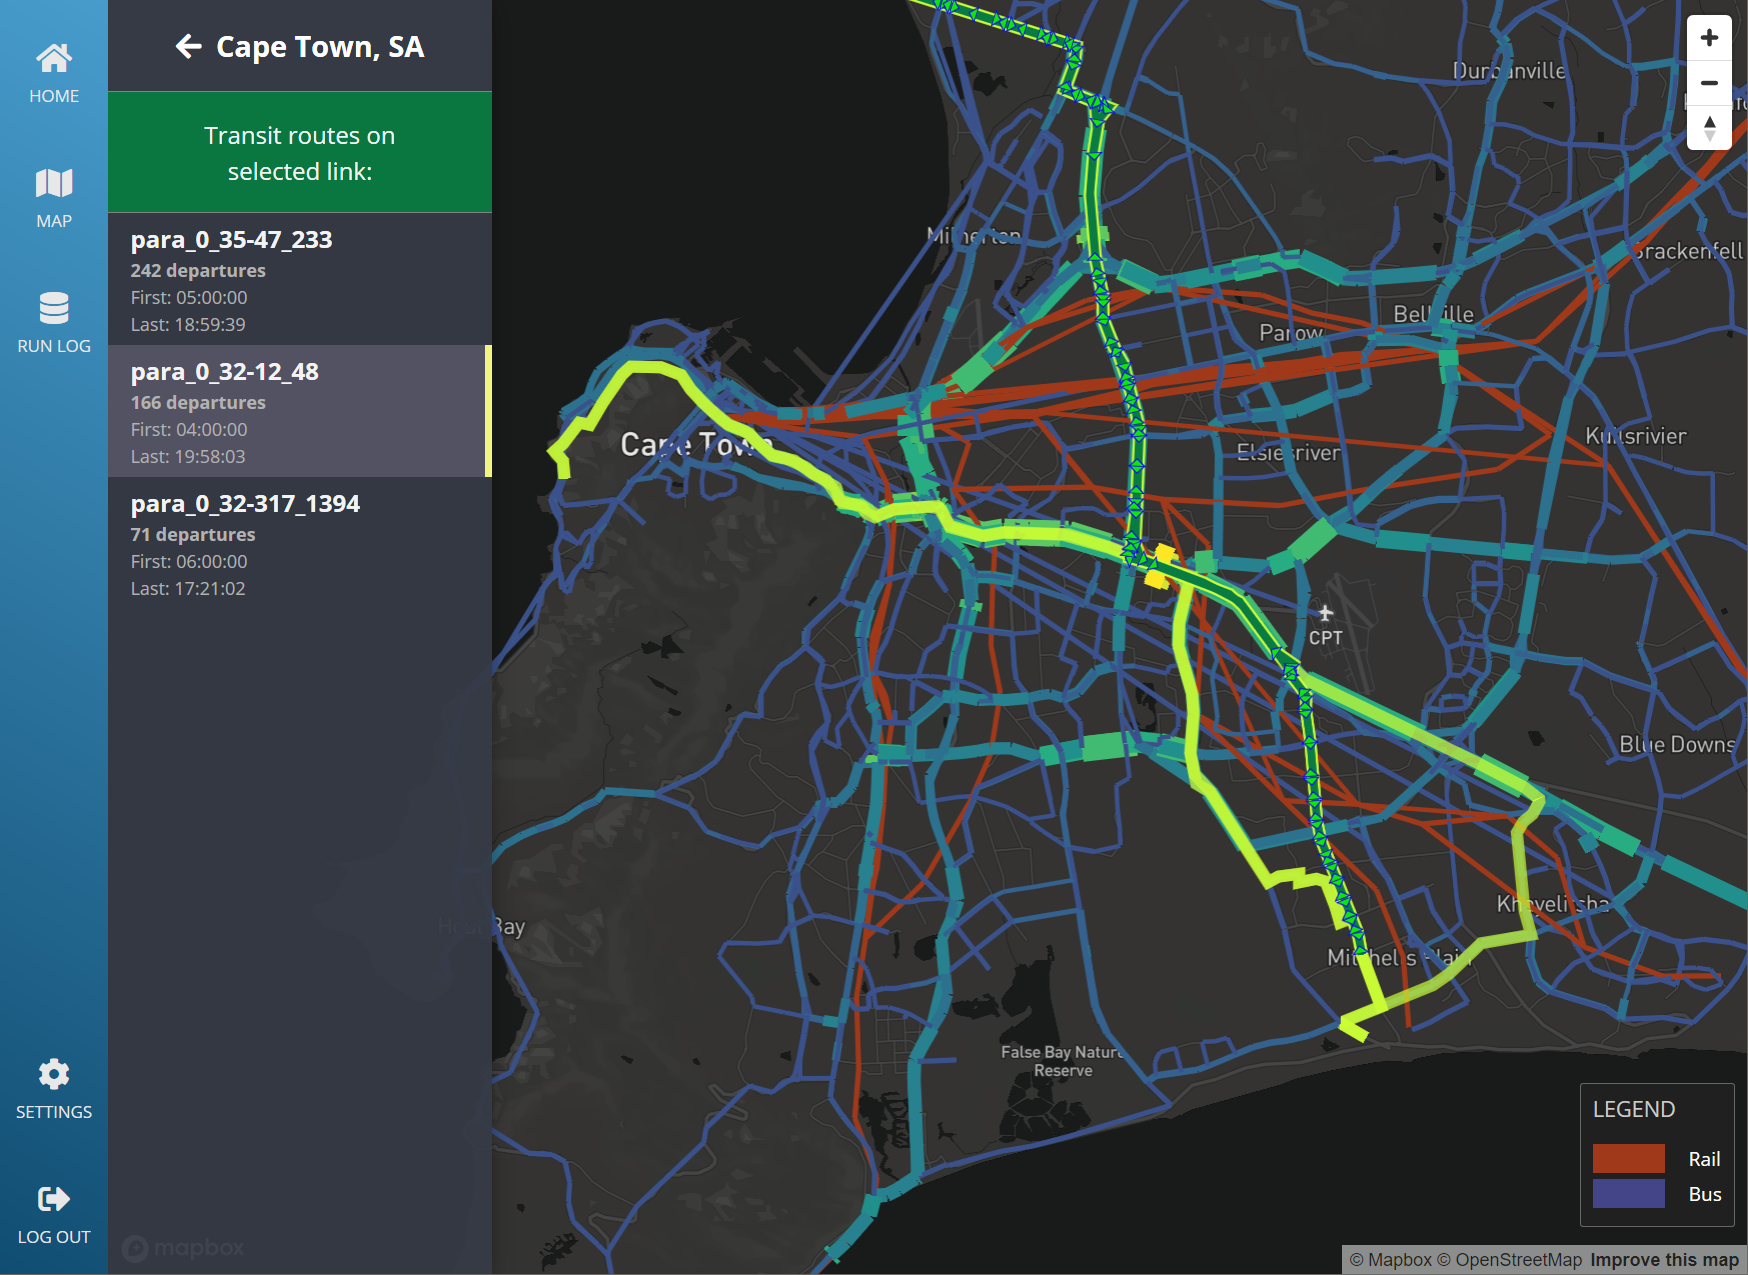
\includegraphics[width=3.25in]{fig-transit.png}
\caption{Transit depiction}\label{Ftransit}
\end{figure}

\begin{figure}
\centering
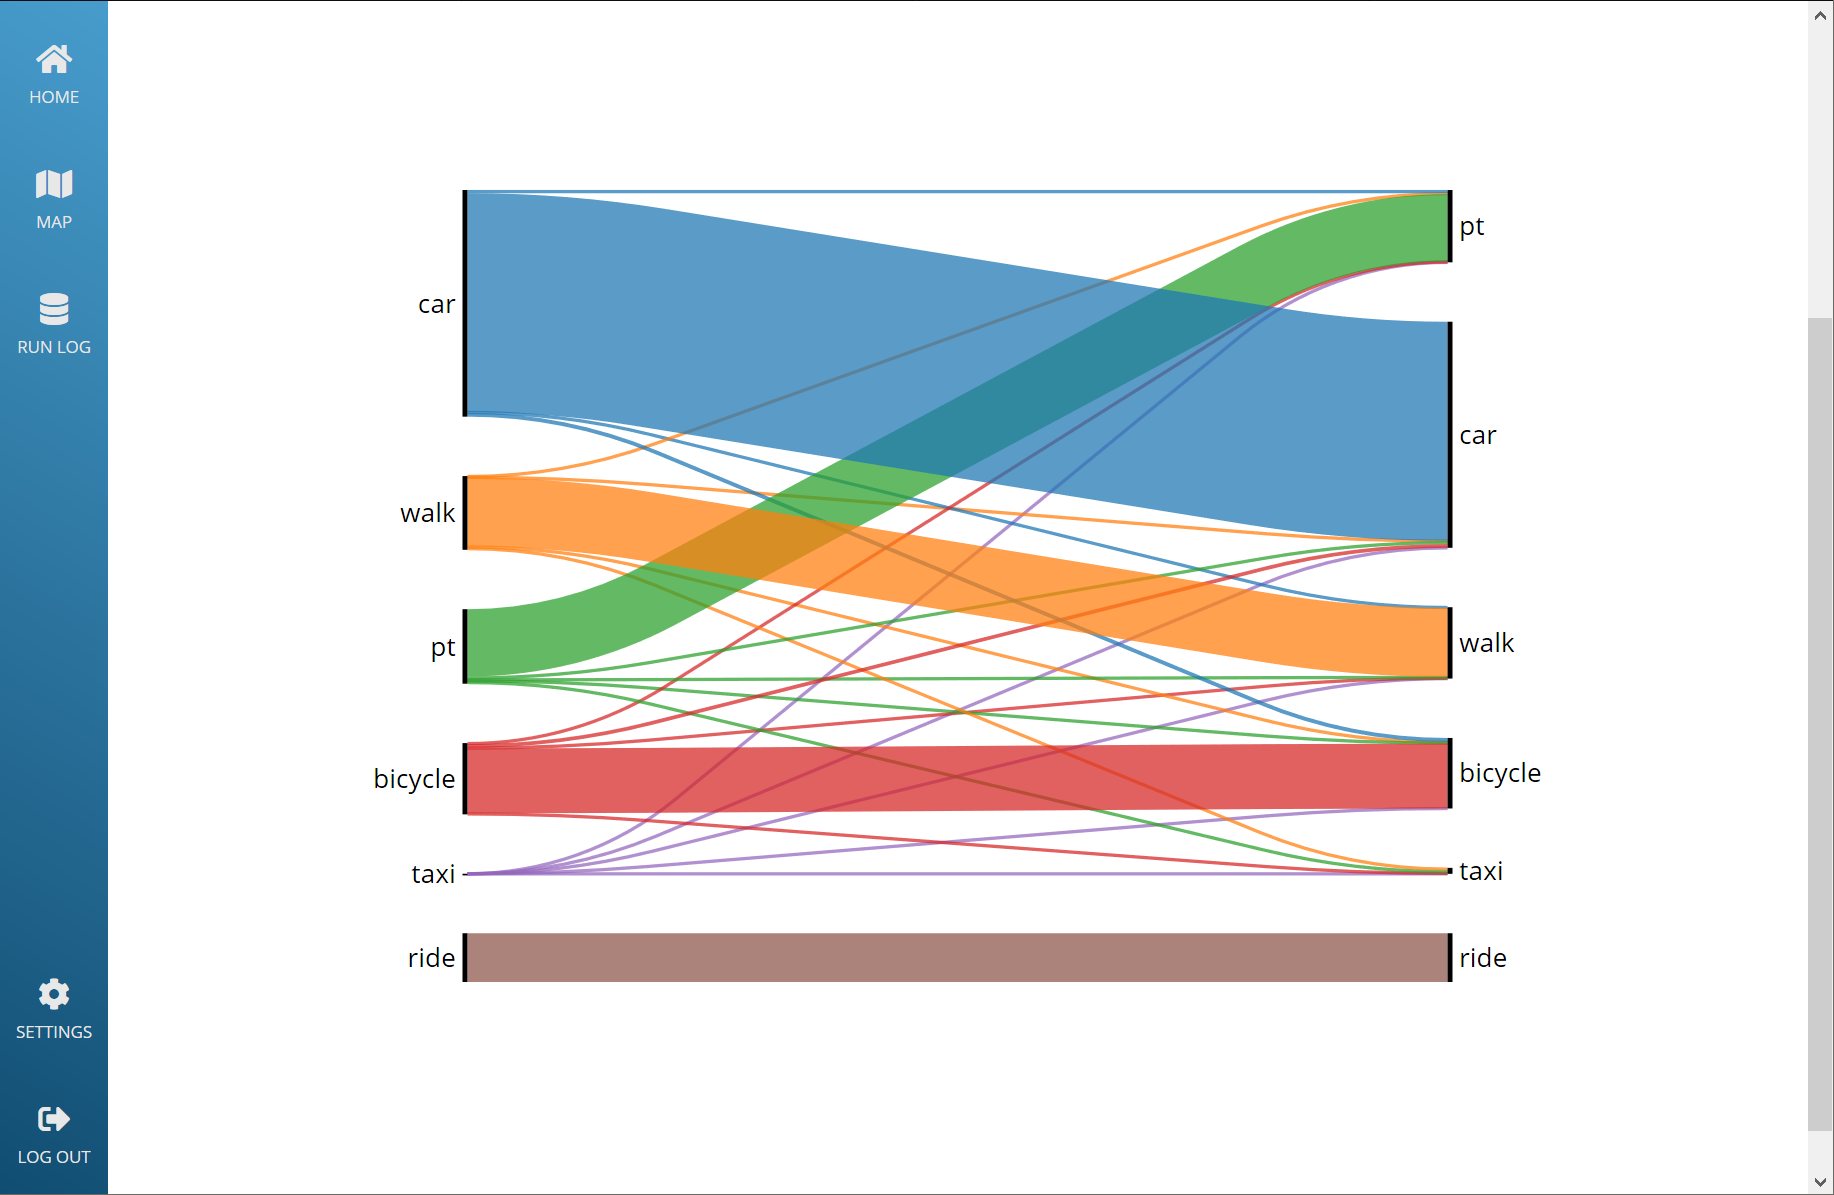
\includegraphics[width=3.25in]{fig-sankey.png}
\caption{Mode shift diagram}\label{Fsankey}
\end{figure}

In addition, one disaggregate animation is available:

\begin{enumerate}
\item[(i)] A vehicle flow simulation, showing individual vehicle agents in real-time on the network. (Figure~\ref{Fanim})
\end{enumerate}

\begin{figure}
\centering
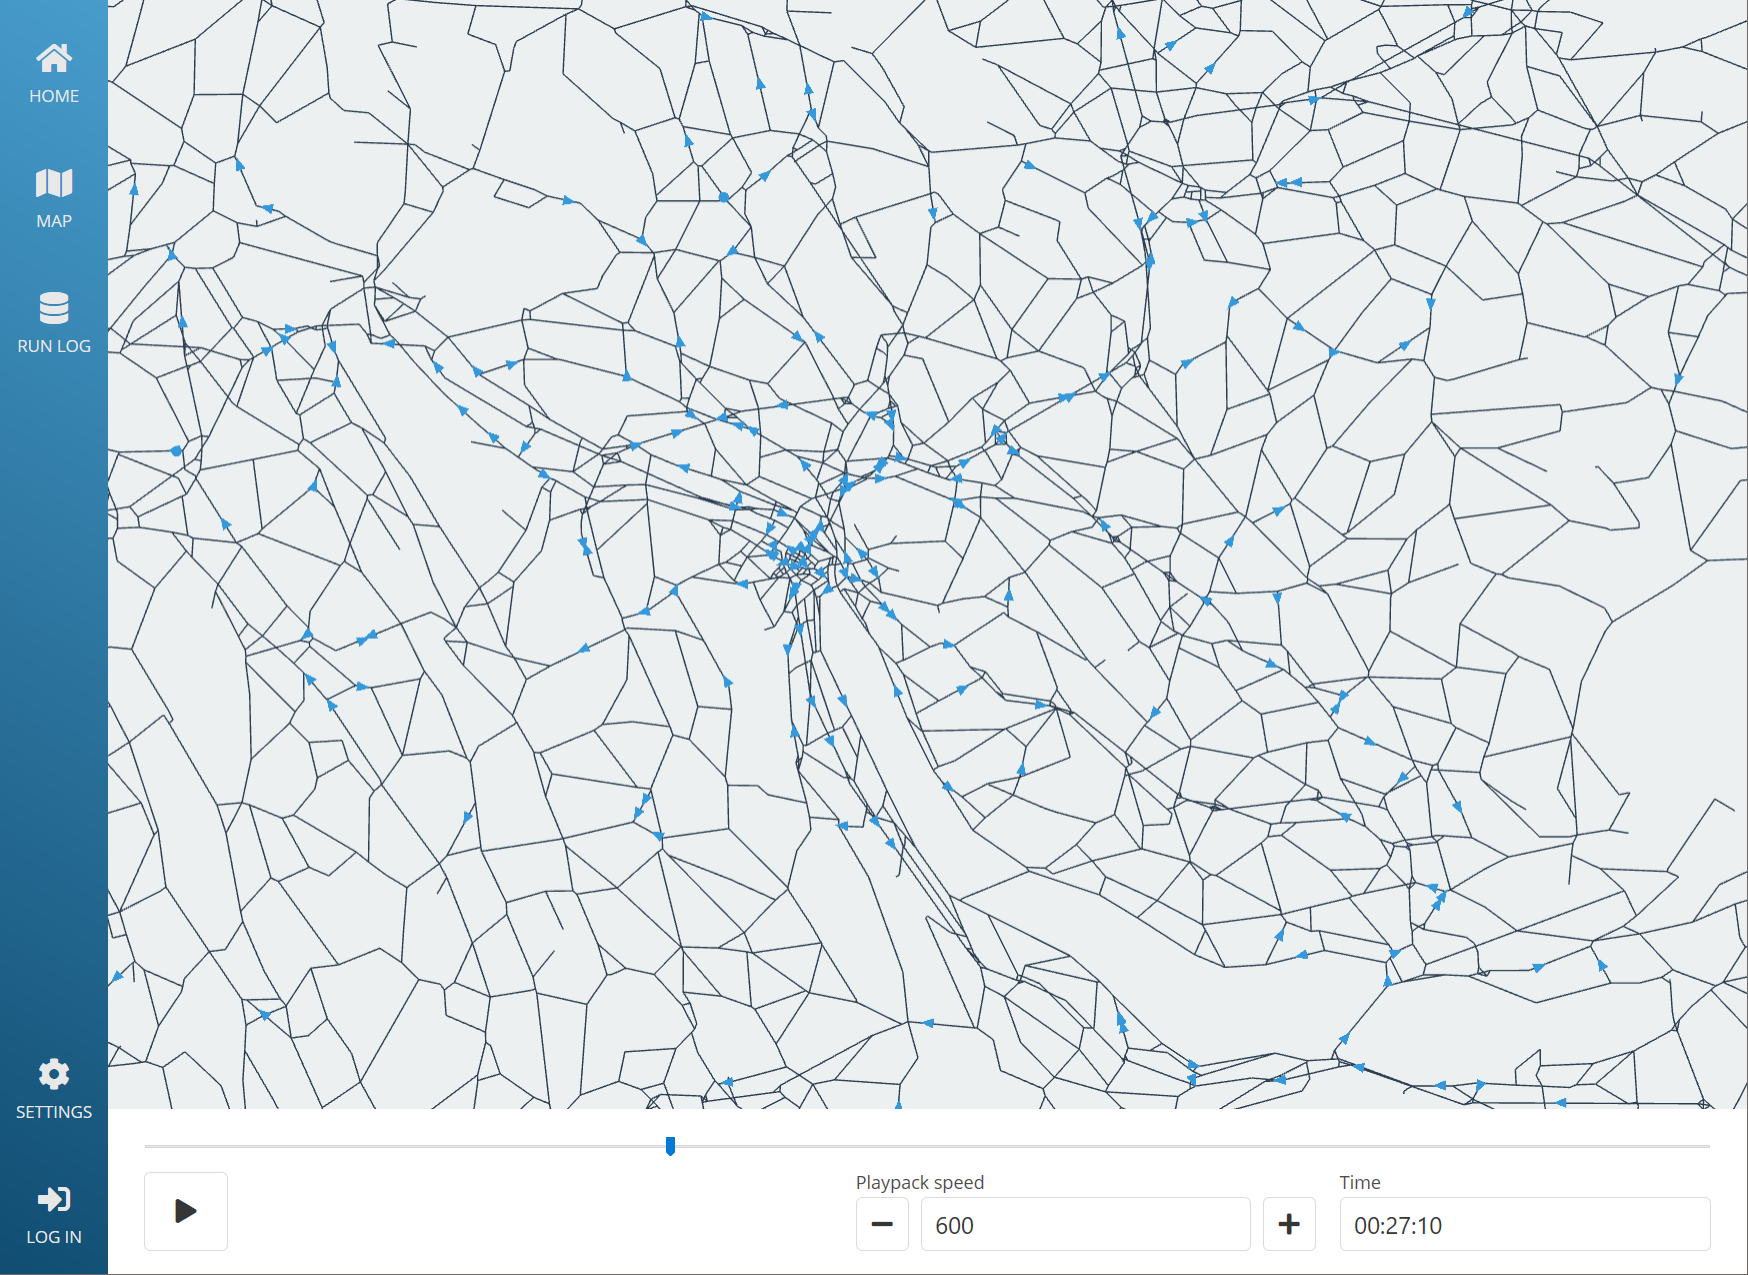
\includegraphics[width=3.25in]{fig-animation.png}
\caption{Vehicle animation}\label{Fanim}
\end{figure}

\subsection{Workflow feedback}

User interface design (UI) and user experience (UX) have their own entire fields of research. Initial prototypes of the tool simply did not meet the needs of test users. Problems included: difficult discerning which files were which; inability to efficiently use the model run tagging feature (in which a user could mark sets of files as belonging to a particular MATSim run); separate user logins causing data to be inaccesible to team members working on the same projects (resulting in everyone using a common "team" login, against best practices); private projects "leaking" onto the public website; and myriad usability bugs in the data visualizations themselves.

These usability problems were eventually solved by surveying other technical websites which organize and present large amounts of data. One website in particular, \url{Github.com}, was found to be well-liked by test users and has a similar hierarchical view of data: users can belong to organizations, and both organizations and users can create projects ("repositories" on Github) which may large numbers of files.

By adopting a file, project, and user paradigm similar to that employed by Github, users were immediately more familiar and had less to learn. The current site adheres to this so closely that test users often refer to the platform as "MatHub".

\subsection{Performance}

Even with modern hardware and the latest browsers, it is quite challenging to produce performant, visually pleasing results with disaggregate MATSim data. The vehicle flow simulation depends heavily on the back-end server to produce and deliver simulation "frames" to the browser in real-time, so that the browser simply has to render the data.

Various levels of aggregation make MATsim data much easier to visualize, as is reflected in the number of different visualizations this research was able to produce with aggregate data in a short time frame.

\textbf{Preprocessing.} The traffic animation and the emissions "hex grid" visualizations both rely on back-end server processes to preprocess the raw MATSim event outputs. This takes anywhere from a few seconds to many minutes, depending on the size of the simulation that was run. The preprocessing only needs to occur once, and thereafter the results are cached and stored on the server. The UI presents a helpful "still processing" message during this stage. Unfortunately, changing some settings such as the size of the hex-grids for the emission tool means the calculations must be redone. Further work is being done to make these processes run as quickly as possible.

\textbf{Map layer limitations.} The Mapbox GL mapping library allows lines, points, and polygons to be displayed on top of a base map. There seems to be a number of map elements beyond which performance becomes very slow; various techniques can be used such as aggregating elements at further-out zoom levels to get around this. Another option is to only use Mapbox GL for the base map, and to use the WebGL graphics libraries to draw large numbers of elements directly on top of the map. This is the technique used for the traffic animation, which can easily support tens of thousands of elements (all in motion!) simultaneously. For additional visualizations which have large numbers of grahical elements, more research will need to be done on layering WebGL elements on top of the base map.

\subsection{Mobile device support}

Initially, the research targeted desktop browsers only. The reasoning was that analysts currently use desktop software, and it would be sufficient to complement those desktop tools with a new web-based option.

However, as the tool started becoming usable by internal users, it quickly became apparent that everyone wanted some version of the visualizations to work on mobile devices, too. It was suggested that even a read-only visualization "viewer" for mobile would be better than not having the tool work at all on mobile.

To address this, the layout of the main user interface needed to be redesigned, but the overall stack of web-based libraries and components chosen was already well-suited to mobile use. This effort is currently underway.

\section{Conclusions and outlook}

Experimenting with the various technologies and getting all of the disparate pieces working together was an enormous task, one which took much longer than anticipated. However, those decisions are now behind us and the platform has become quite stable.

A new visualization can now be generated by the researchers in a matter of days or weeks. The researchers are admittedly very familiar with the inner workings of the system, but even so it has been encouraging to see new visualizations go from ideation to rough draft in such a short time.

None of the above-listed visualizations are particularly groundbreaking or visually stunning. And, all of them could be easily created in other tools (although usually without the interactivity that the web enables). This is a bit disappointing but the open nature of the platform, requiring no software installation by end users, still has an advantage: it opens up the display of MATSim results to the public and to decisionmakers, even if they do not have access to desktop mapping or travel forecasting software.

Another use case that has emerged from these visualization experiments is a more regimented data management tool for MATSim. Currently there is no straightforward way to share MATSim datasets online. The combination of the new file storage and management capabilities along with the Github-like user interface provides a natural place for users to store and disseminate results.

Importantly, the world has not stood still while this platform was under development. Just in the past year, major data visualization efforts from well-funded companies such as Uber and others have been released. There are legitimate questions about how much of this work could be superceded by large, well-funded, professional coding teams.

Despite these concerns, the MATSim visualization framework is operational and is now just beginning to be useful for researchers at the department of its creation. This bodes well for further development in the near future.

All code is available on the MATSim Github site, at \url{github.com/matsim-org/viz}.

% -------------------------------------------------------------

\begin{acks}
This research project is part of the National Research Programme "Big Data" (NRP 75) of the Swiss National Science Foundation.\\
Website: \url{http://www.nrp75.ch/}
\end{acks}

\begin{thebibliography}{99}

\bibitem[Horni, A., Nagel, K., \& Axhausen, K. W. (Eds.). (2016)]{R1}
Horni, A., Nagel, K., \& Axhausen, K. W. (Eds.). (2016). \textit{The multi-agent transport simulation MATSim} (p. 618). London: Ubiquity Press.

\bibitem[Strippgen, David (2016)]{R2}
Strippgen, David (2016) \textit{OTFVis: MATSim’s Open-Source Visualizer}. In Andreas Horni, Kai Nagel, Kay W. Axhausen (Eds.): The Multi-Agent Transport Simulation MATSim: Ubiquity Press, pp. 225–234.

\bibitem[Rieser, Marcel (2016)]{R3}
Rieser, Marcel (2016) \textit{Senozon Via}. In Andreas Horni, Kai Nagel, Kay W. Axhausen (Eds.): The Multi-Agent Transport Simulation MATSim: Ubiquity Press, pp. 219–224.

\bibitem[Free Software Soundation (2007)]{R4}
Free Software Soundation (2007) \textit{GNU General Public License}, Version 3.
URL: www.gnu.org/licenses/gpl.html

\bibitem[Satyanarayan, A., Moritz, D., Wongsuphasawat, K., and Heer, J. (2016)]{R5}
Satyanarayan, A., Moritz, D., Wongsuphasawat, K., and Heer, J. (2016) \textit{Vega-Lite: A Grammar of Interactive Graphics}. IEEE Transactions on Visualization and Computer Graphics, Volume 23, Issue 1. DOI: doi.org/10.1109/TVCG.2016.2599030

\bibitem[Wilkinson, Leland (2005)]{R6}
Wilkinson, Leland (2005) \textit{The Grammar of Graphics}, Second Edition. Springer Press, Chicago, USA. DOI: doi.org/10.1007/0-387-28695-0

\end{thebibliography}

\end{document}
